\changelocaltocdepth{0}

\chapter{Open Questions and Conjectures}
\label{ch:conjectures}

This chapter summarizes some open questions and conjectures arising from the computer search and findings in the previous chapters.

\section{Enumeration of levelable graphs} In \autoref{sec:enumeration} we presented a table showing the number of levelable graphs on $n \leq 10$ vertices. For larger graphs, checking the levelable condition becomes computationally burdensome due to the large linear system and the number of connected graphs. It remains an open question how the number of levelable graphs grows with the number of vertices.

\begin{question}
For $n > 10$, how many graphs on $n$ vertices are levelable?
\end{question}

\section{Caterpillar Graphs} In \autoref{sec:caterpillar}, we introduced caterpillar graphs, which are special tree graphs where all vertices are at most distance 1 from a central path. In \autoref{thm:caterpillar} we showed that if every vertex on the central path contains at least one ``leg'' vertex, then the graph most be levelable. The data generated from the computer search suggest that this is also a necessary condition, since all levelable caterpillars on 10 or fewer vertices satisfy this ``minimum leg condition.'' We therefore state the converse statement of \autoref{thm:caterpillar} as the following conjecture:

\begin{conjecture}
A caterpillar graph $G$ is levelable if and only if every vertex on the central path (except for perhaps the endpoints of the path) has at least one leg vertex. 
\end{conjecture}

\section{Graph Expansions}
First, recall from \autoref{thm:expansion} that performing a uniform graph expansion on a levelable graph produces a new levelable graph. That is, the levelablity of a graph is preserved if we replace each vertex with an independent set of some size $k \geq 1$. However, we have not yet addressed a general graph expansion on $G$ where the $n$ vertices $V(G) = \br{v_1, \dots, v_n}$ are replaced with independent sets of size $k_1, \dots, k_n$ respectively. Are there weaker conditions on $k_1, \dots, k_n$ or the graph $G$ that still preserves the levelability of a graph? In other words:

\begin{question}
For a levelable graph $G$, under what conditions is a non-uniform expansion of $G$ also levelable?
\end{question}

\section{Adding vertices to levelable graphs} In \autoref{sec:adding-vertices-levelable}, we proved that given a levelable graph $G$ with maximal independent sets $F_1, \dots, F_t$, we can construct a new levelable graph by adding $m \leq \max\br{|F_i|}$ new vertices adjacent to all existing vertices. However, this bound on $m$ arose out of convenience with respect to the system in \autoref{thm:level-condition}. Therefore, it is likely there are cases in which we can relax this bound, which raises the following question:

\begin{question}
For a levelable graph $G$ with maximal independent sets $F_1, \dots, F_t$, under what conditions does adding $m > \max\br{|F_i|}$ completely connected vertices produce a levelable graph?
\end{question}

\section{Adding vertices to non-levelable graphs} \label{sec:question-adding-non} \autoref{thm:adding-vertices-non-levelable} states that adding vertices that are adjacent to at least one vertex in each facet of a non-levelable graph yields a new non-levelable graph. Is the converse statement true? We pose this as an open question:
\begin{question}
Let $G$ be a non-levelable graph with a vertex $v'$ such that $v'$ is adjacent to all maximal independent sets of $G$. Let $G'$ denote the induced subgraph $G'$ with $V(G') = V(G) \setminus \br{v'}$ and $E(G') = E(G) \setminus \br{\br{v', w} \; | \; \br{v', w} \in E(G)}$. Is $G'$ also non-levelable?
\end{question}

In this report we have also explored cases in which the addition of vertices does not satisfy the condition in \autoref{thm:adding-vertices-non-levelable} but still results in a non-levelable graph (e.g. adding a vertex to the 5-path to create the 6-path). There are also cases where the resulting graph is levelable (e.g. the graph in \autoref{ex:5-path-induce}, where one vertex was added to the path to create a 3-cycle). It is therefore an interesting problem to relax this condition for \autoref{thm:adding-vertices-non-levelable}, as well as identify where we can add vertices to make a non-levelable path graph levelable.
\begin{question}
If $G$ is the path graph on $n$ vertices, where must vertices and edges be added to make the resulting graph levelable?
\end{question}
\noindent
More generally, we ask:
\begin{question}
If $G$ is a non-levelable graph, what graph operations make the resulting graph levelable?
\end{question}

\section{Other criteria on vertex partitions} \label{sec:other-criteria}
In \autoref{thm:graph-partitions}, we showed that we can preclude levelability if the vertex set of a graph can be partitioned in a certain way such that certain unions of the partitioning sets are maximal independent sets. This criterion was based on the independent sets of the path on 5 vertices. In \autoref{ex:5-path} we formally showed the non-existence of a valid solution to the system for the path on 5 vertices, and the proof \autoref{thm:graph-partitions} depended on a similar contradiction. In the latter, the partition sets of the vertex set ``represented" the vertices of the path. Can we exploit the independent set structure of other non-levelable to construct new criteria in a similar way to \autoref{thm:graph-partitions}? We leave this as an open problem: 
\begin{question} 
Do there exist other paritions of $V(G)$ similar to \autoref{thm:graph-partitions} that prevent a graph from being levelable?
\end{question}
\noindent
We can think of the 5-path as being the ``minimal" case of \autoref{thm:graph-partitions}, since this is the case where each partition set contains only one vertex. Since the path on 6 vertices cannot be partitioned to satisfy \autoref{thm:graph-partitions}, we expect that this will yield a different partition condition. However, the paths on 7 vertices or greater are covered by the condition in \autoref{thm:graph-partitions} arising from the 5-path. We can therefore see that there is some minimal set of non-levelable graphs that give rise to a unique set of conditions that preclude levelability. 

For example, for graphs on 5 vertices, this set is trivial since there is only one non-levelable graph. Hence the path on 5 vertices gives a condition that trivially captures all non-levelable graphs on 5 vertices. However, for 6 vertices we need at least two unique conditions. The non-levelable graph $G$ on 6 vertices $V(G) = \br{v_1, \dots, v_6}$ and edge set 
$$
E(G) = \br{\br{v_i, v_{i+1}} \; | \; i = 1, \dots, 4} \cup \br{\br{v_4, v_6}}
$$
can be partitioned according to \autoref{thm:graph-partitions} (see \autoref{fig:6-vertex}), while the (non-levelable) path on 6 vertices is the minimal case of a new condition. 

\begin{figure}[bth]
    \myfloatalign
    \subfloat
    {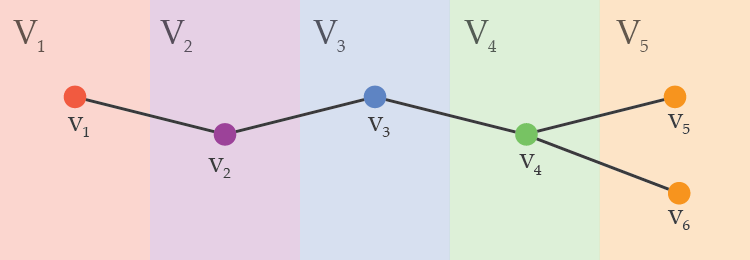
\includegraphics[width=.7\linewidth]{figures/6-vertex-1.png}} \\ \vspace{1cm}
    \subfloat
    {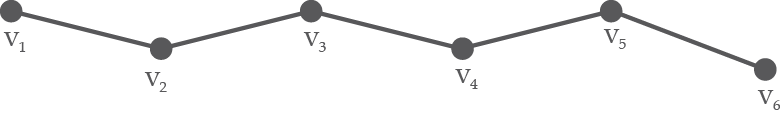
\includegraphics[width=.7\linewidth]{figures/6-path.png}} 
    \caption{An example of a graph on 6 vertices (top) that satisfies \autoref{thm:graph-partitions}, with the vertices coloured to illustrate the partition; and the path on 6 vertices (bottom), which cannot be partitioned in this way.} \label{fig:6-vertex}
\end{figure}
\noindent
This observation raises the following question:
\begin{question}
How many unique partition conditions are required to capture all non-levelable graphs on $n$ vertices?
\end{question}



